\chapter{\MakeUppercase{Resultados Experimentais}}\label{sec:resultados}

Este capítulo apresenta os resultados na ordem das questões de pesquisa. A \autoref{sec2:res-rq1} avalia o componente preditivo; a \autoref{sec2:res-rq2} apresenta o \textit{backtest} financeiro; a \autoref{sec2:res-rq3} apresenta a análise de sensibilidade. Todos os experimentos foram executados em 23 de setembro de 2026 com a configuração descrita no \autoref{sec:configuracao}. O caso base do motor prescritivo usa armazenagem de 2,50 R\$/sc/mês, quebra técnica de 0,2 \%/mês, taxa de desconto de 10 \% a.a., neutralidade a risco ($\lambda = 0$) e \textit{hedge} habilitado; a Selic vigente em cada data é tratada como um dos cenários de sensibilidade.

\section{Resultados para a RQ1: acurácia preditiva}\label{sec2:res-rq1}

\subsection{LSTM contra os métodos de referência}

A \autoref{tab:rq1-metricas} apresenta as métricas da rede e dos três métodos de referência nos conjuntos de validação e de teste, por horizonte. As métricas de erro estão no espaço do log-retorno; o MAPE é o erro percentual equivalente no preço reconstruído.

\begin{table}[htb]
	\centering
	\caption{Acurácia por horizonte nos conjuntos de validação (372 amostras) e teste (417 amostras). RMSE e MAE em log-retorno; MAPE em \% do preço; direção em \% de acertos de sinal.}\label{tab:rq1-metricas}
	\footnotesize
	\setlength{\tabcolsep}{3.5pt}
	\begin{tabular}{l l r r r r r r r}
		\hline
		\textbf{Conjunto} & \textbf{Horiz.} & \multicolumn{4}{c}{\textbf{LSTM}} & \multicolumn{3}{c}{\textbf{RMSE das referências}} \\
		& & RMSE & MAE & MAPE & Direção & Passeio aleat. & ARIMA(1,1,2) & Curva futuros \\ \hline
		Validação & 21 d  & 0,112 & 0,081 & 8,7  & 55,6 & \textbf{0,091} & \textbf{0,090} & 0,107 \\
		          & 63 d  & 0,194 & 0,158 & 17,6 & 60,8 & 0,177 & 0,177 & \textbf{0,156} \\
		          & 126 d & \textbf{0,185} & 0,152 & 16,8 & 77,2 & 0,236 & 0,236 & 0,193 \\ \hline
		Teste     & 21 d  & 0,147 & 0,112 & 10,6 & 58,3 & \textbf{0,120} & \textbf{0,119} & 0,130 \\
		          & 63 d  & \textbf{0,213} & 0,150 & 13,9 & 71,5 & 0,233 & 0,233 & 0,227 \\
		          & 126 d & \textbf{0,267} & 0,192 & 16,9 & 79,1 & 0,321 & 0,321 & 0,309 \\ \hline
	\end{tabular}
	\fonte{Do autor (2026).}
\end{table}

Três padrões emergem. Primeiro, no horizonte de 21 dias a LSTM perde para o passeio aleatório e para o ARIMA nos dois conjuntos: no curto prazo, a melhor previsão do log-retorno é zero, e qualquer modelo que tente prever direção paga em variância. Segundo, o ARIMA é indistinguível do passeio aleatório em todos os horizontes, com RMSE igual até a terceira casa decimal e acerto direcional próximo de 50 \%, o que confirma que a série diária de log-preço é quase integrada e que o passeio aleatório é a referência estatística adequada. Terceiro, a vantagem da LSTM cresce com o horizonte: em 126 dias ela vence todas as referências nos dois conjuntos, com acerto direcional de 77 \% na validação e 79 \% no teste.

A curva de futuros ajustada pela base sazonal é a referência mais exigente. Na validação ela supera a LSTM em 21 e 63 dias e empata em 126. No teste, período de volatilidade recorde, a curva perde poder preditivo (acerto direcional de 42 a 61 \%) e a LSTM passa a vencê-la em 63 e 126 dias. Em termos de erro absoluto, todas as abordagens pioram do conjunto de validação para o de teste, reflexo do regime de preços sem precedente no período.

A \autoref{fig:previsto-realizado} mostra o previsto contra o realizado por horizonte no conjunto de teste e evidencia a principal deficiência do modelo: a compressão das previsões em direção a zero. As previsões raramente ultrapassam $\pm 0{,}2$ em log-retorno, enquanto os retornos realizados de 126 dias chegaram a $+0{,}57$ na alta do segundo semestre de 2024. A rede acerta a direção, mas subestima a magnitude dos movimentos extremos.

\begin{figure}[htb]
	\centering
	\caption{Log-retorno previsto contra realizado por horizonte no conjunto de teste.}\label{fig:previsto-realizado}
	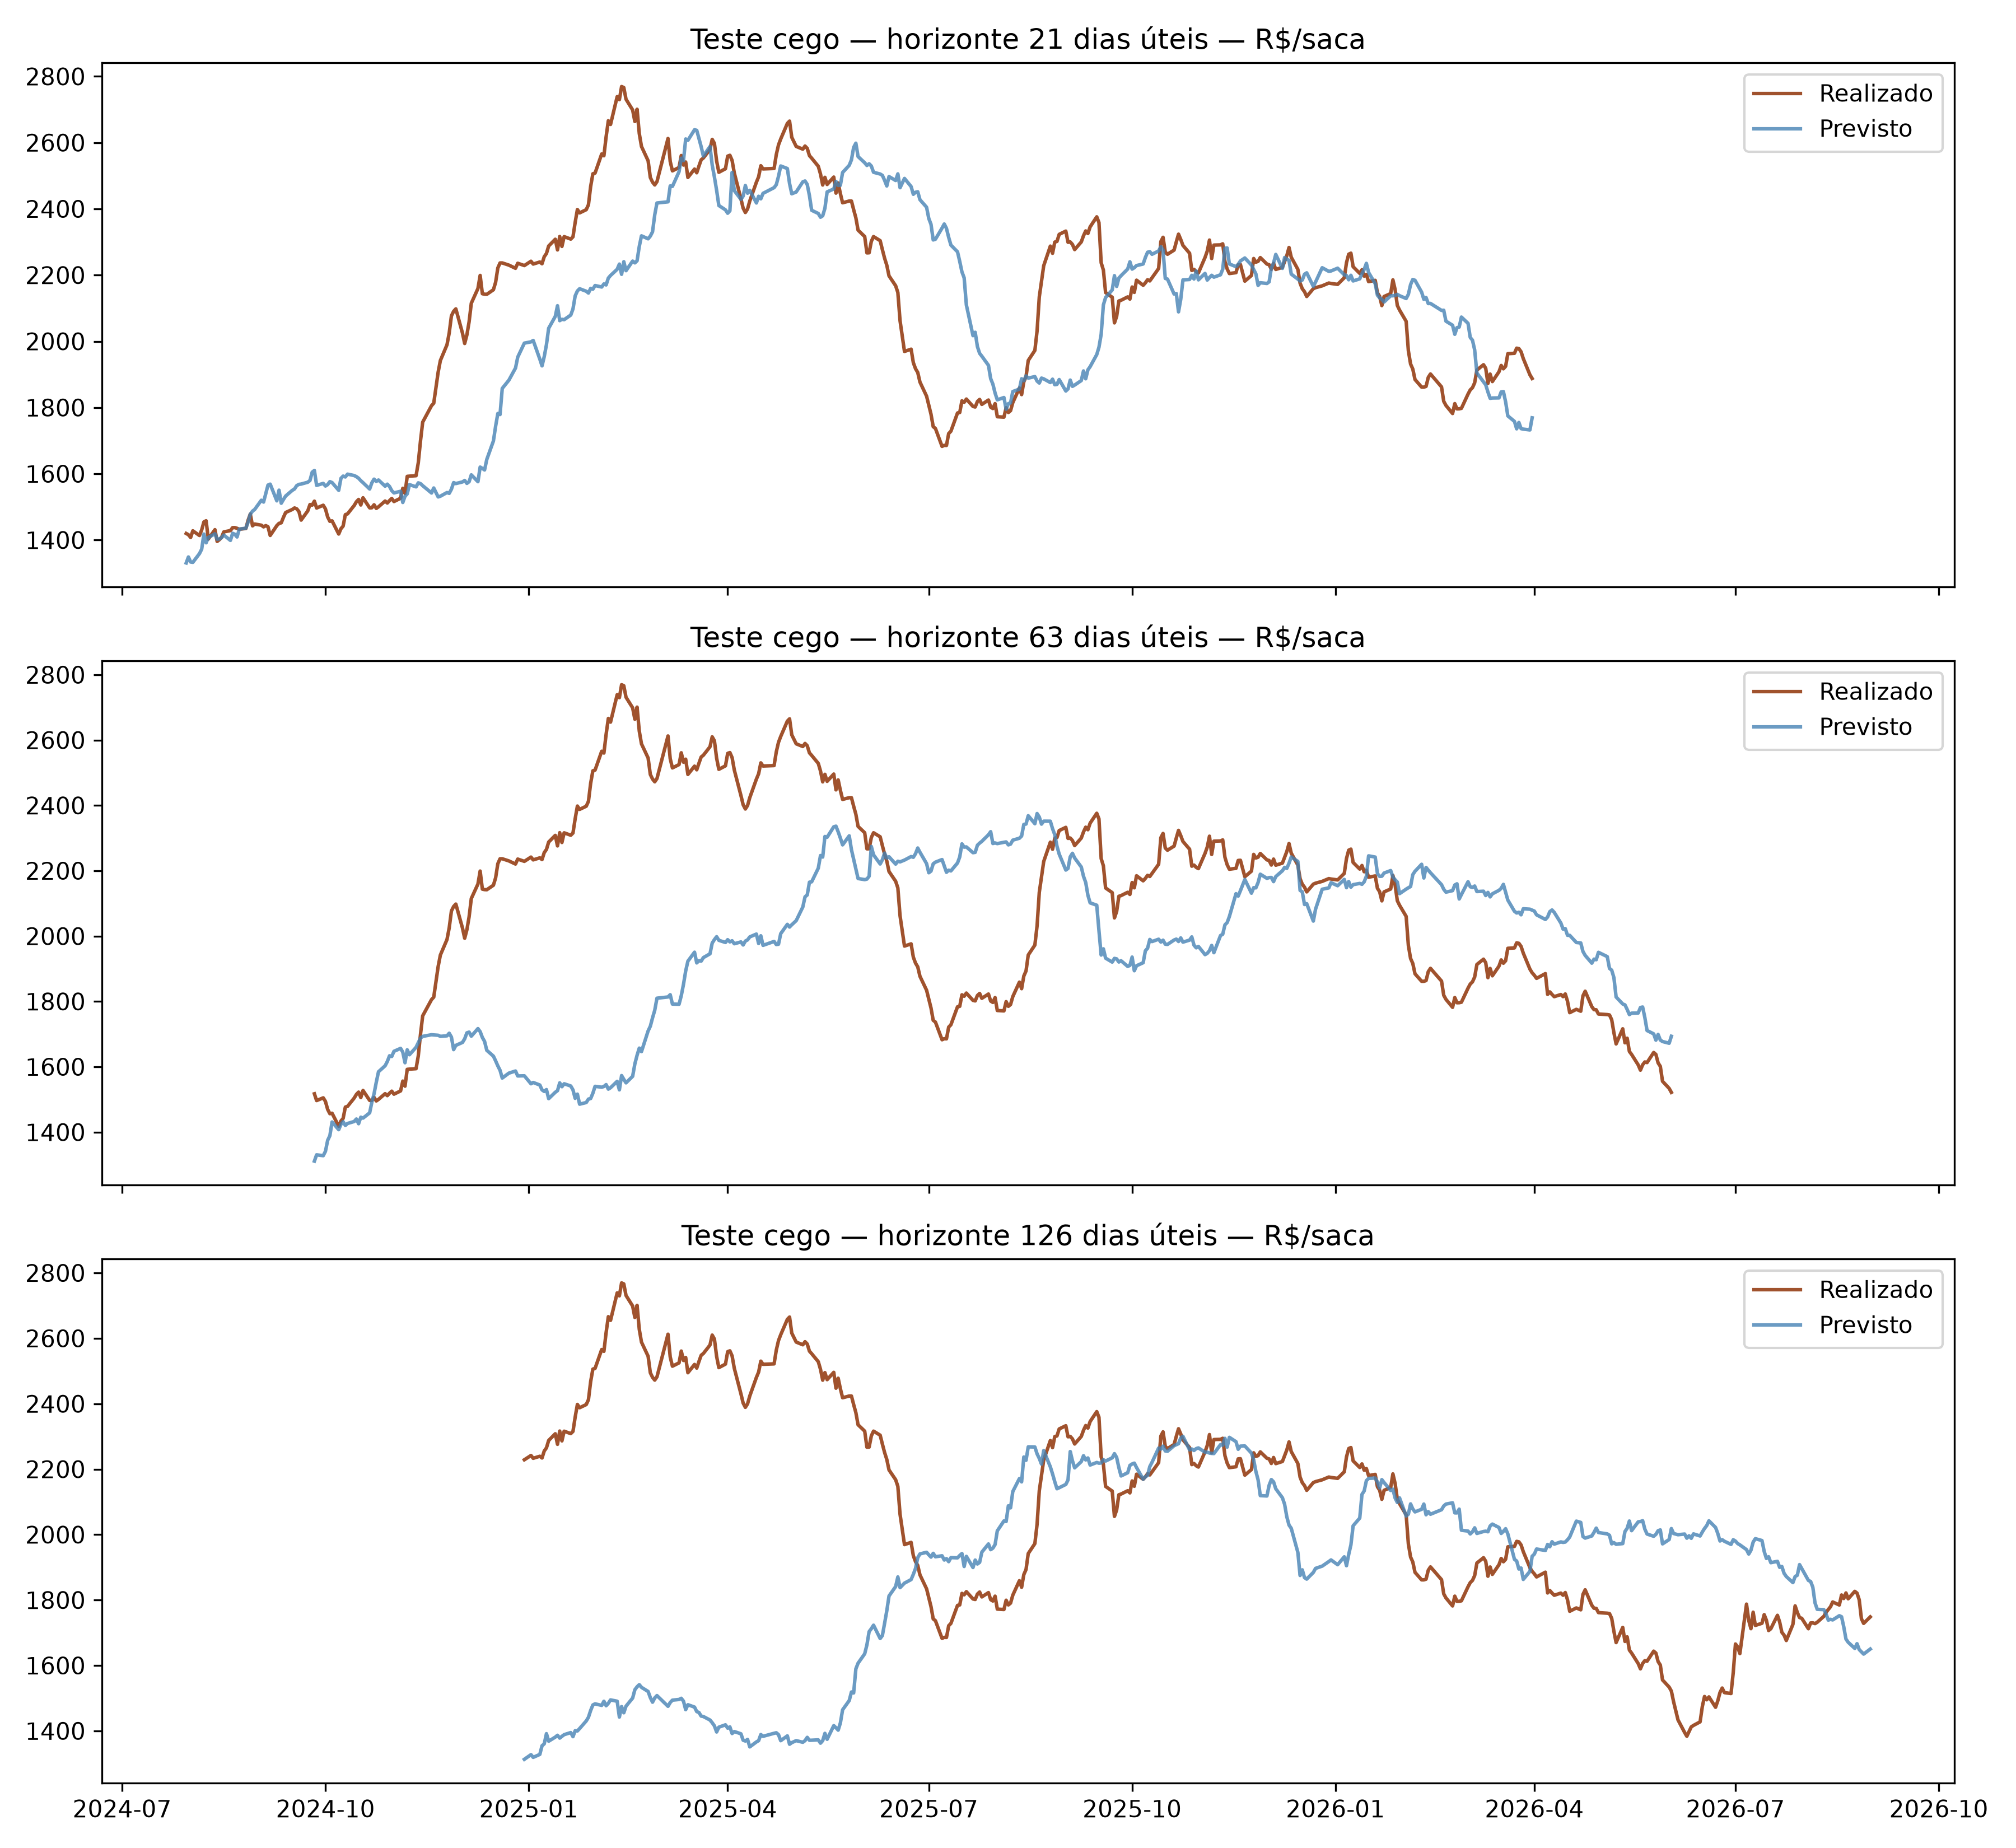
\includegraphics[width=\textwidth]{imgs/03_previsto_realizado_teste.png}
	\fonte{Do autor (2026).}
\end{figure}

\subsection{Variabilidade entre inicializações}

Antes de interpretar diferenças entre modelos é preciso conhecer a variabilidade do próprio treino. O modelo completo foi treinado com cinco sementes distintas; a \autoref{tab:rq1-seeds} resume o resultado na validação.

\begin{table}[htb]
	\centering
	\caption{Variabilidade do modelo completo entre cinco sementes (validação).}\label{tab:rq1-seeds}
	\begin{tabular}{l r r r}
		\hline
		\textbf{Métrica} & \textbf{Média} & \textbf{Desvio} & \textbf{Semente 42 (modelo final)} \\ \hline
		RMSE 21 d  & 0,114 & 0,008 & 0,112 \\
		RMSE 63 d  & 0,188 & 0,017 & 0,194 \\
		RMSE 126 d & 0,192 & 0,024 & 0,185 \\
		Direção 21 d (\%)  & 56,9 & 4,0 & 55,6 \\
		Direção 63 d (\%)  & 61,5 & 6,3 & 60,8 \\
		Direção 126 d (\%) & 74,1 & 8,2 & 77,2 \\ \hline
	\end{tabular}
	\fonte{Do autor (2026).}
\end{table}

O modelo final está dentro de um desvio-padrão da média em todas as métricas: não é o melhor nem o pior sorteio. A vantagem da curva de futuros sobre a LSTM na validação, de 0,008 em 21 dias e 0,032 em 63 dias, é da ordem de um desvio no primeiro caso e de quase dois no segundo. A diferença em 63 dias é, portanto, robusta à inicialização; a de 21 dias, não.

\subsection{Estudo de ablação}

Cada um dos seis grupos de variáveis foi removido por vez, e a rede foi retreinada com três sementes por configuração. A \autoref{tab:rq1-ablacao} apresenta a variação relativa do RMSE médio em relação ao modelo completo; valores positivos indicam que remover o grupo piorou o erro.

\begin{table}[htb]
	\centering
	\caption{Ablação por grupo de variáveis: variação relativa do RMSE médio de três sementes em relação ao modelo completo (validação). Positivo indica piora ao remover o grupo.}\label{tab:rq1-ablacao}
	\footnotesize
	\setlength{\tabcolsep}{4pt}
	\begin{tabular}{l r r r r}
		\hline
		\textbf{Grupo removido} & \textbf{$\Delta$ 21 d} & \textbf{$\Delta$ 63 d} & \textbf{$\Delta$ 126 d} & \textbf{Dir. 126 d} \\ \hline
		Nenhum (completo)          & ---     & ---    & ---     & 71,3 \% \\
		(a) Retornos e médias móveis & $-$10,1 \% & $-$6,9 \% & $-$10,0 \% & 77,4 \% \\
		(b) Mercado (vol., spread, base) & $-$6,7 \% & $-$8,3 \% & $+$10,4 \% & 59,5 \% \\
		(c) Calendário e Selic     & $+$3,9 \%  & $-$3,1 \% & $+$11,7 \% & 66,8 \% \\
		(d) Clima                  & $+$3,5 \%  & $+$6,1 \% & $-$9,4 \%  & 73,2 \% \\
		(e) Fundos (COT)           & $+$1,4 \%  & $-$6,5 \% & $-$12,4 \% & 75,8 \% \\
		(f) Insumos                & $+$7,2 \%  & $-$7,0 \% & $-$11,4 \% & 83,9 \% \\ \hline
	\end{tabular}
	\fonte{Do autor (2026).}
\end{table}

O desvio entre sementes dentro de cada configuração é de 2 a 5 \% do RMSE em 21 e 63 dias e de cerca de 11 \% em 126 dias, de modo que apenas efeitos acima dessa ordem merecem interpretação. Com esse critério, a ablação sustenta quatro conclusões.

\begin{alineas}
	\item Os grupos de \textbf{mercado} e de \textbf{calendário e Selic} são os que carregam sinal de longo prazo: removê-los piora o RMSE de 126 dias em 10 a 12 \% e derruba o acerto direcional nesse horizonte de 71 \% para 59 \% e 67 \%.
	\item O \textbf{clima} contribui nos horizontes de 21 e 63 dias, com piora de 3 a 6 \% ao ser removido, mas não em 126 dias.
	\item Remover \textbf{retornos e médias móveis}, \textbf{fundos} ou \textbf{insumos} melhora o erro de 126 dias em 10 a 12 \%. Esses grupos, no modelo completo, adicionam mais ruído que informação no horizonte longo.
	\item A ablação não sustenta a hipótese de que todas as variáveis exógenas contribuem para a acurácia. Sustenta que um subconjunto (mercado, calendário, Selic e clima) é essencial e que uma versão enxuta do modelo é candidata natural para reduzir o sobreajuste discutido no \autoref{sec:discussao}.
\end{alineas}

\section{Resultados para a RQ2: ganho financeiro da prescrição}\label{sec2:res-rq2}

\subsection{Backtest no teste cego}

A \autoref{tab:rq2-teste} apresenta a receita líquida média por saca, em valor presente, das sete estratégias nas 20 datas de decisão do teste cego, separadas por safra. A \autoref{fig:receita-por-data} mostra a receita de cada estratégia em cada data.

\begin{table}[htb]
	\centering
	\caption{Receita líquida média por saca (R\$, valor presente) no teste cego, por safra.}\label{tab:rq2-teste}
	\footnotesize
	\setlength{\tabcolsep}{3.5pt}
	\begin{tabular}{l r r r r r r r r}
		\hline
		\textbf{Safra} & \textbf{n} & \textbf{Imed.} & \textbf{Parc.} & \textbf{M. móvel} & \textbf{Meta COE} & \textbf{Hedge} & \textbf{AgroVis.} & \textbf{Oráculo} \\ \hline
		2024/25 & 12 & 1\,999 & \textbf{2\,057} & 1\,996 & 1\,999 & 1\,805 & 2\,003 & 2\,418 \\
		2025/26 & 8  & 2\,072 & 1\,919 & 1\,963 & 2\,072 & 2\,076 & \textbf{2\,199} & 2\,202 \\
		Total   & 20 & 2\,028 & 2\,001 & 1\,983 & 2\,028 & 1\,913 & \textbf{2\,081} & 2\,331 \\ \hline
	\end{tabular}
	\fonte{Do autor (2026).}
\end{table}

\begin{figure}[htb]
	\centering
	\caption{Receita líquida por data de decisão no teste cego, todas as estratégias.}\label{fig:receita-por-data}
	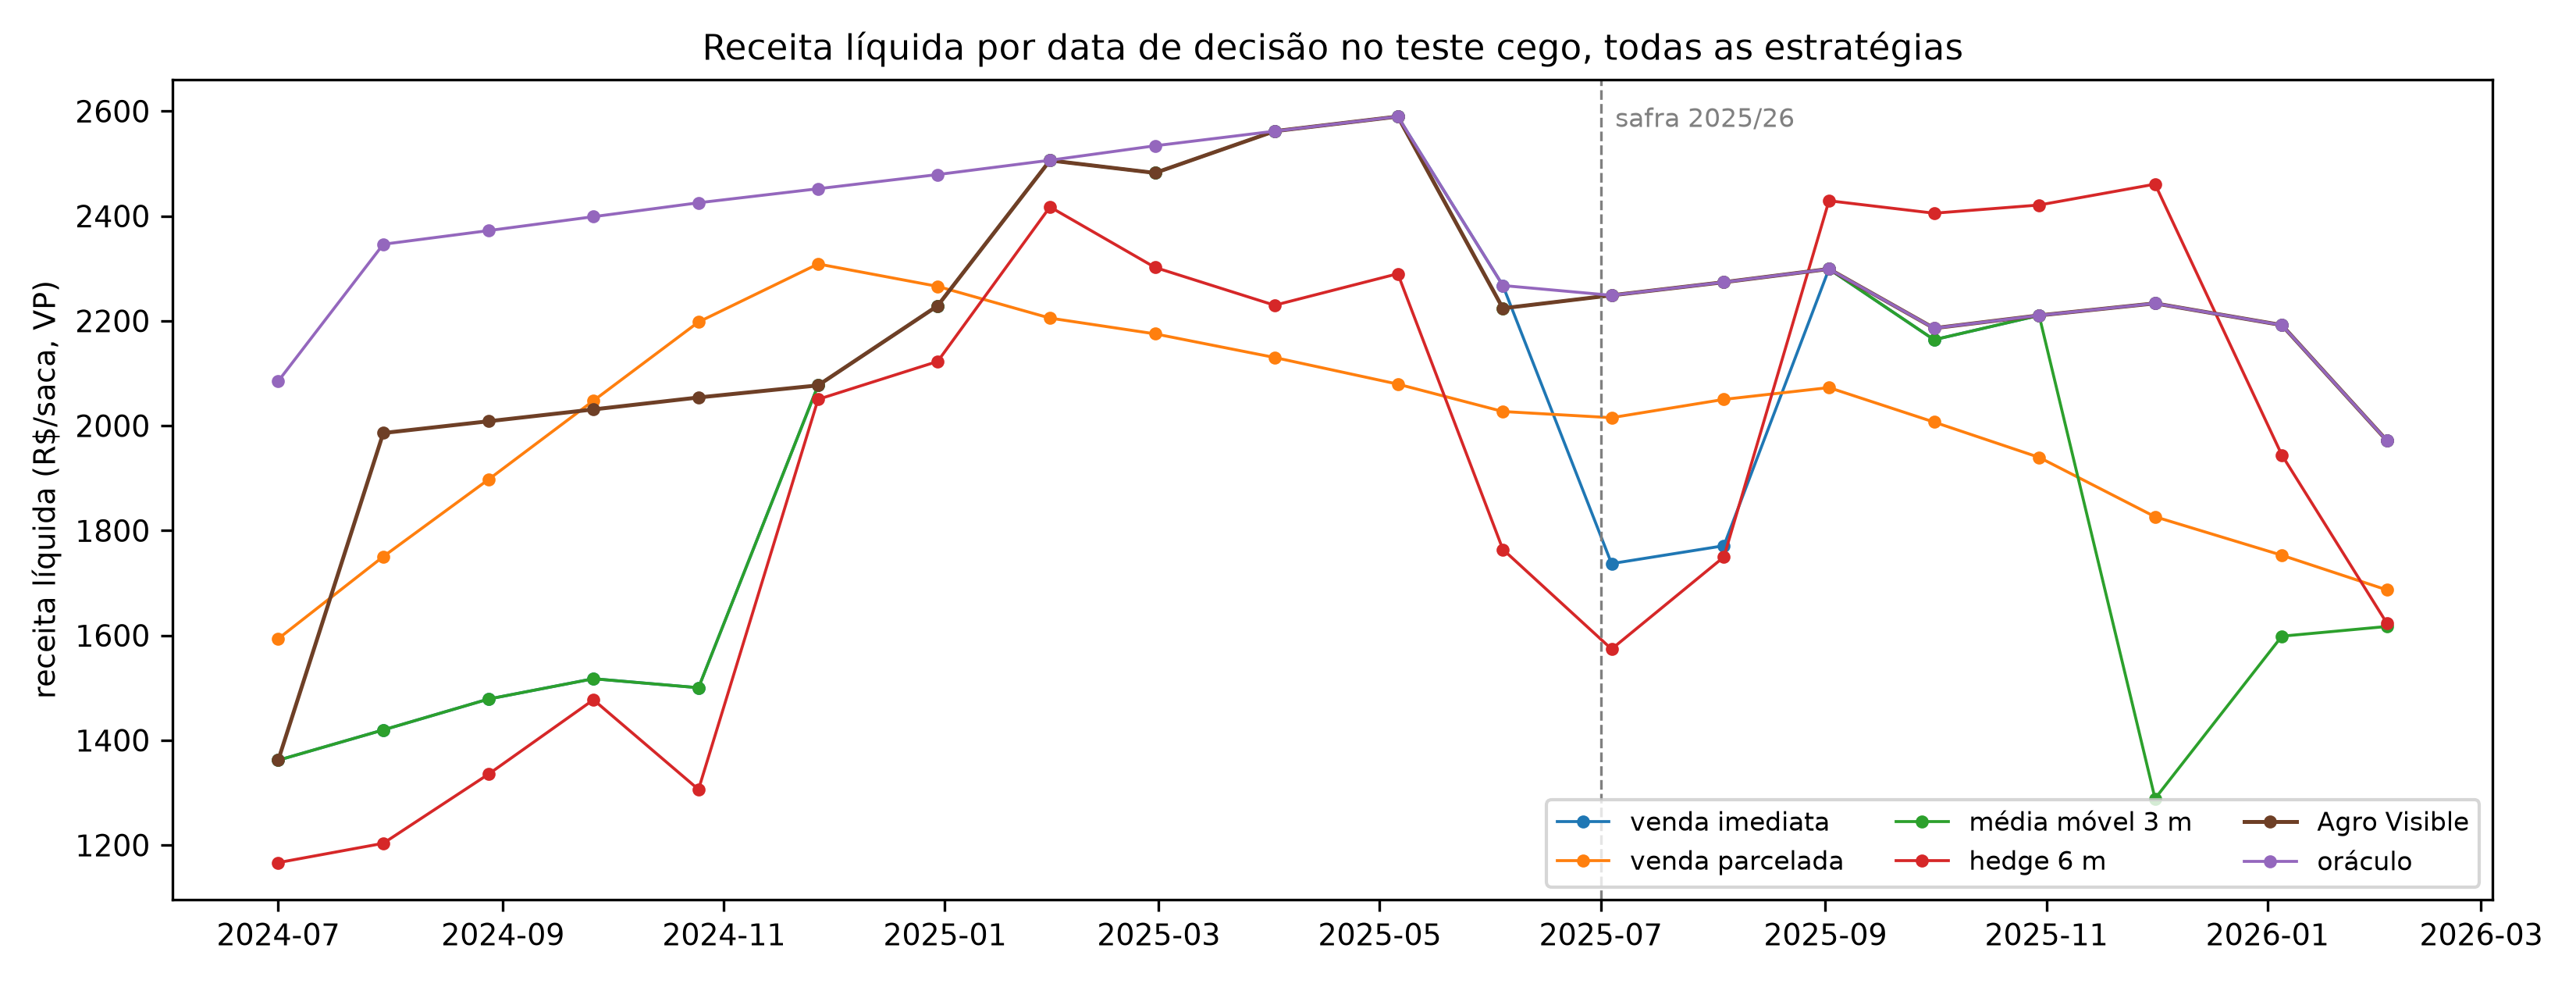
\includegraphics[width=\textwidth]{imgs/07_receita_por_data_teste.png}
	\fonte{Do autor (2026).}
\end{figure}

No agregado das 20 datas, o AgroVisible obteve 2\,081 R\$/sc contra 2\,028 da venda imediata, ganho de 2,6 \%, e contra 2\,001 da venda parcelada, ganho de 4,0 \%. As duas safras, porém, contam histórias opostas.

Na safra 2024/25 o café subiu de 1\,362 R\$/sc em julho de 2024 para mais de 2\,500 em janeiro de 2025, uma alta de 84 \% em seis meses. A estratégia vencedora foi a venda parcelada, que diluiu a venda ao longo da alta sem precisar prevê-la. O AgroVisible armazenou em julho e agosto de 2024, mas vendeu após um ou dois meses com ganhos de 4 \% e 1 \%, e vendeu imediatamente de setembro a dezembro porque a previsão de 21 dias era negativa em todas essas datas, enquanto o retorno realizado de 126 dias foi superior a 50 \%. O modelo não enxergou a alta persistente, e a compressão das previsões para zero fez o motor abandonar o estoque cedo. O resultado ficou praticamente igual ao da venda imediata.

Na safra 2025/26 ocorreu o oposto. Em julho e agosto de 2025, com o preço em torno de 1\,750 R\$/sc após uma queda de 30 \%, a rede previu recuperação, o motor armazenou por dois meses e um mês, respectivamente, e a receita foi 29 \% e 28 \% superior à venda imediata, capturando 100 \% do ganho do oráculo nessas datas. No platô alto que se seguiu, vender imediatamente era ótimo e foi o que o motor fez. A safra fechou em 2\,199 R\$/sc contra 2\,072 da venda imediata, a três reais do oráculo.

O \textit{hedge} de seis meses foi a pior estratégia no teste, com perda de 5,7 \% contra a venda imediata, porque o mercado esteve em \textit{backwardation} durante quase todo o período: vender o futuro travava um preço abaixo do físico. A meta de margem sobre o COE coincidiu com a venda imediata em todas as datas, pois o preço nunca esteve abaixo de 1,3 vez o COE. O motor nunca escolheu a ação de \textit{hedge} no \textit{backtest}, e a receita do AgroVisible com e sem essa ação é idêntica no teste.

\subsection{Ampliação da amostra ao período de validação}

Vinte decisões em duas safras de alta histórica constituem uma amostra pequena e atípica. O mesmo protocolo foi aplicado às 18 datas de decisão do período de validação, de julho de 2022 a dezembro de 2023, que inclui uma queda de 40 \% no preço. Nessas duas safras a dispersão residual e a parada antecipada da rede foram calibradas com os próprios dados, o que introduz um viés favorável leve à LSTM; as estatísticas de base já eram estimadas apenas no treino. A \autoref{tab:rq2-4safras} apresenta o resultado por safra e o consolidado de 38 datas.

\begin{table}[htb]
	\centering
	\caption{Receita líquida média por saca (R\$, valor presente) nas quatro safras. As safras 2022/23 e 2023/24 pertencem ao período de validação.}\label{tab:rq2-4safras}
	\footnotesize
	\setlength{\tabcolsep}{3.5pt}
	\begin{tabular}{l r r r r r r r r}
		\hline
		\textbf{Safra} & \textbf{n} & \textbf{Imed.} & \textbf{Parc.} & \textbf{M. móvel} & \textbf{Meta COE} & \textbf{Hedge} & \textbf{AgroVis.} & \textbf{Oráculo} \\ \hline
		2022/23 & 12 & \textbf{1\,139} & 992 & 1\,101 & \textbf{1\,139} & 1\,051 & 1\,106 & 1\,160 \\
		2023/24 & 6  & 853 & 919 & 859 & 922 & 758 & \textbf{958} & 1\,026 \\
		2024/25 & 12 & 1\,999 & \textbf{2\,057} & 1\,996 & 1\,999 & 1\,805 & 2\,003 & 2\,418 \\
		2025/26 & 8  & 2\,072 & 1\,919 & 1\,963 & 2\,072 & 2\,076 & \textbf{2\,199} & 2\,202 \\ \hline
		Total   & 38 & 1\,562 & 1\,512 & 1\,527 & 1\,573 & 1\,459 & \textbf{1\,596} & 1\,755 \\
		Ganho s/ imediata & & --- & $-$1,6\,\% & $-$1,7\,\% & $+$1,3\,\% & $-$7,7\,\% & $+$2,7\,\% & $+$14,0\,\% \\
		Captura oráculo & & 90,0\,\% & 86,5\,\% & 87,9\,\% & 91,1\,\% & 83,3\,\% & 91,9\,\% & 100\,\% \\ \hline
	\end{tabular}
	\fonte{Do autor (2026).}
\end{table}

Na safra 2022/23, de queda, o AgroVisible perdeu 3 \% para a venda imediata. Duas decisões em maio e junho de 2023 explicam quase toda a perda: a rede previu alta, o motor armazenou até o fim do horizonte e o preço caiu 20 \%, com perdas de 25 \% e 28 \% nessas datas. Na safra 2023/24, de recuperação a partir de um fundo, o motor armazenou em todas as datas e venceu todas as heurísticas, com ganho de 12 \% sobre a venda imediata.

No consolidado de quatro safras e dois regimes, o AgroVisible foi a única estratégia a superar a venda imediata em todos os agregados, com ganho de 2,7 \% e captura de 91,9 \% do valor do oráculo. A venda parcelada, que venceu na safra de alta, perdeu 1,6 \% no consolidado, porque carrega estoque durante as quedas. A \autoref{tab:rq2-oraculo} mostra a fração do ganho disponível capturada por cada estratégia nas datas em que o oráculo superava a venda imediata em mais de 1 \%, isto é, nas datas em que havia algo a ganhar armazenando.

\begin{table}[htb]
	\centering
	\caption{Fração do ganho do oráculo capturada, (estratégia $-$ imediata)/(oráculo $-$ imediata), média nas datas em que armazenar era vantajoso.}\label{tab:rq2-oraculo}
	\begin{tabular}{l r r}
		\hline
		\textbf{Estratégia} & \textbf{Teste (n = 11)} & \textbf{Quatro safras (n = 21)} \\ \hline
		Venda parcelada & $-$79,0 \% & $-$52,1 \% \\
		Média móvel 3 m & 18,2 \% & 28,3 \% \\
		Meta de margem COE & 0,0 \% & 15,1 \% \\
		Hedge 6 m & 51,7 \% & $-$22,7 \% \\
		AgroVisible & 19,0 \% & \textbf{47,4 \%} \\ \hline
	\end{tabular}
	\fonte{Do autor (2026).}
\end{table}

\subsection{Significância estatística}

A \autoref{tab:rq2-estatistica} apresenta a diferença pareada por data entre o AgroVisible e as duas heurísticas nomeadas na RQ2, com intervalo de confiança de 95 \% por \textit{bootstrap} de 10\,000 reamostragens e p-valor do teste de Wilcoxon pareado.

\begin{table}[htb]
	\centering
	\caption{Diferença pareada de receita por data (R\$/sc) entre o AgroVisible e as heurísticas.}\label{tab:rq2-estatistica}
	\footnotesize
	\setlength{\tabcolsep}{3.5pt}
	\begin{tabular}{l r l r r r r}
		\hline
		\textbf{Amostra} & \textbf{n} & \textbf{Comparação} & \textbf{Média} & \textbf{IC 95 \%} & \textbf{p (Wilcoxon)} & \textbf{Datas positivas} \\ \hline
		Teste & 20 & vs. imediata  & 52,8 & [$-$0,1; 128,6] & 0,271 & 20 \% \\
		Teste & 20 & vs. parcelada & 79,8 & [$-$76,0; 221,5] & 0,294 & 65 \% \\
		Quatro safras & 38 & vs. imediata  & 34,0 & [$-$6,8; 79,9] & 0,066 & 34 \% \\
		Quatro safras & 38 & vs. parcelada & 84,0 & [$-$3,1; 163,2] & \textbf{0,018} & 71 \% \\ \hline
	\end{tabular}
	\fonte{Do autor (2026).}
\end{table}

No teste isolado nenhuma diferença é significativa ao nível de 5 \%, o que era esperado com 20 observações e desvio-padrão da diferença de 156 R\$/sc. Com as 38 datas, a vantagem sobre a venda parcelada torna-se significativa ($p = 0{,}018$) e a vantagem sobre a venda imediata fica na margem ($p = 0{,}066$), com intervalo de confiança que inclui o zero por pouco. A baixa fração de datas positivas contra a venda imediata (34 \%) decorre da própria estrutura da política: na maioria das datas o motor vende imediatamente e a diferença é zero. O ganho concentra-se em poucas decisões de armazenar com retorno elevado, o que torna a média positiva mas a mediana nula, e é isso que o teste de Wilcoxon penaliza.

\subsection{Anatomia das decisões}

A \autoref{fig:gatilho} ilustra a saída do motor para a data de 31 de agosto de 2026, a mais recente disponível: para cada mês futuro, o preço a partir do qual vender é ótimo. Nos dois primeiros meses o gatilho está acima de 3\,000 R\$/sc, ou seja, a política é armazenar em quase qualquer cenário; do terceiro mês em diante o gatilho cai abaixo do preço corrente e a venda passa a ser recomendada assim que o preço previsto se estabiliza. Essa forma de política, armazenar enquanto a deriva prevista supera o custo de carregamento e vender quando ela se esgota, é a regra que o produtor recebe da ferramenta, e não uma única data de venda.

\begin{figure}[htb]
	\centering
	\caption{Gatilho de venda por mês para a decisão de 31 de agosto de 2026: preço a partir do qual vender é ótimo, contra o preço previsto.}\label{fig:gatilho}
	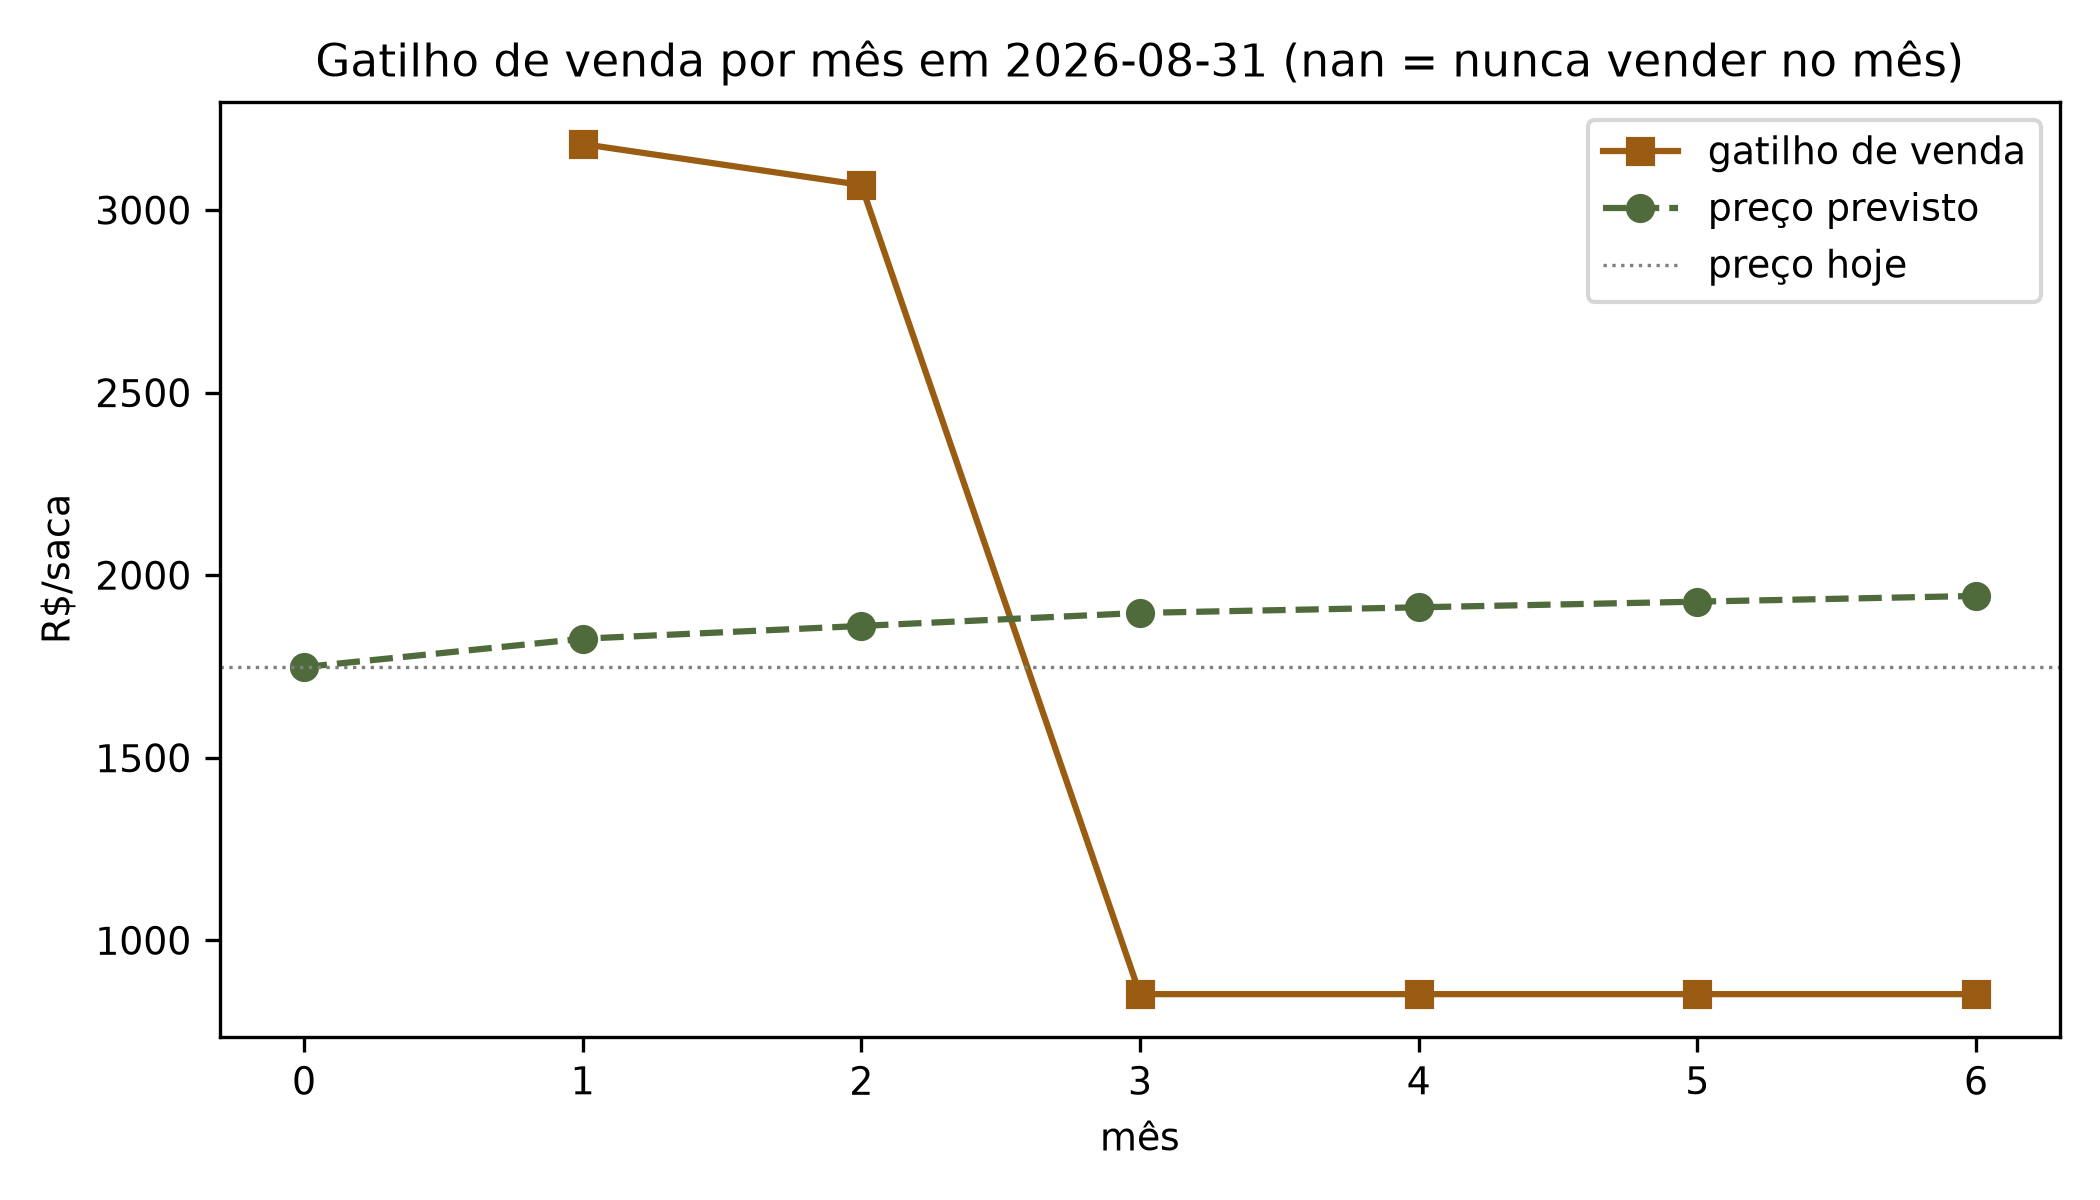
\includegraphics[width=0.85\textwidth]{imgs/06_gatilho_venda_por_mes.png}
	\fonte{Do autor (2026).}
\end{figure}

A decomposição por data das 38 decisões mostra que os quatro maiores ganhos (julho e agosto de 2025, julho e outubro de 2023) vieram de previsões de alta de 21 dias corretas em direção, e que as duas maiores perdas (maio e junho de 2023) vieram de previsões de alta erradas em datas de queda forte. Em cinco das 38 datas o motor armazenou e a venda imediata teria sido melhor; em treze, armazenou e ganhou; nas vinte restantes vendeu de imediato. O ganho médio positivo vem, portanto, de uma assimetria: quando o motor acerta a recuperação a partir de um fundo, o ganho é de 10 a 30 \%; quando erra, a perda média é menor, porque a política rolante revende o estoque assim que a previsão do mês seguinte deixa de justificar o carregamento.

\subsection{O custo operacional efetivo no motor}

O COE real por safra foi obtido da série histórica de custos de produção da CONAB para o café arábica em Guaxupé, Minas Gerais: 766, 714, 784 e 876 R\$/sc para as safras de 2022 a 2025. O valor provisório de 700 R\$/sc estava dentro da faixa. Com esses valores, a margem mínima observada sobre o COE no teste foi de 74 \%, e a restrição de não vender abaixo de COE$\times$(1 + m) não atuou em nenhuma data para m até 30 \%. No período de validação, com preços entre 800 e 1\,200 R\$/sc, a heurística de meta de margem passou a diferir da venda imediata em 7 das 18 datas e obteve 1\,062 contra 1\,043 R\$/sc. A restrição foi mantida como parâmetro opcional, desligada por padrão: ela só altera a decisão quando o preço está abaixo do piso, e nesse caso força o produtor a carregar o café justamente quando o modelo prevê queda, o que configura regra de sobrevivência financeira e não política de comercialização. A sinalização de margem e a classificação do resultado esperado nas faixas de lucro do módulo de custos, por sua vez, acompanham toda recomendação.

\section{Resultados para a RQ3: robustez da política}\label{sec2:res-rq3}

A \autoref{tab:rq3} consolida a sensibilidade da política aos parâmetros econômicos, no \textit{backtest} do teste cego. A \autoref{fig:sensibilidade} mostra o mapa de calor de aversão a risco contra armazenagem e a curva de sensibilidade à taxa de desconto.

\begin{table}[htb]
	\centering
	\caption{Sensibilidade da política no teste cego (20 datas). Receita do AgroVisible em R\$/sc; frequência de armazenar em \% das datas; datas em que a ação em $k = 0$ muda em relação ao caso base.}\label{tab:rq3}
	\footnotesize
	\setlength{\tabcolsep}{3.5pt}
	\begin{tabular}{l l r r r}
		\hline
		\textbf{Parâmetro} & \textbf{Valor} & \textbf{Receita} & \textbf{Freq. armazenar} & \textbf{Ações alteradas} \\ \hline
		Taxa de desconto & 8 \% a.a.   & 2\,083 & 25 \% & 0 \\
		                 & 10 \% (base) & 2\,081 & 25 \% & --- \\
		                 & 12 \%       & 2\,080 & 25 \% & 0 \\
		                 & 15 \%       & 2\,078 & 25 \% & 0 \\
		                 & Selic vigente por data & 2\,079 & 25 \% & 0 \\ \hline
		Armazenagem      & 1,50 R\$/sc/mês & 2\,082 & 25 \% & 0 \\
		                 & 5,00 R\$/sc/mês & 2\,080 & 25 \% & 0 \\ \hline
		Base esperada    & $-$5 pp / $+$5 pp & 2\,081 & 25 \% & 0 \\
		Risco de base    & $\times 2$   & 2\,081 & 25 \% & 0 \\ \hline
		Aversão a risco $\lambda$ & 0,25 & 2\,080 & 15 \% & 2 \\
		                 & 0,50 & 2\,079 & 10 \% & 3 \\
		                 & 1,00 & 2\,029 & 5 \%  & 4 \\ \hline
	\end{tabular}
	\fonte{Do autor (2026).}
\end{table}

\begin{figure}[htb]
	\centering
	\caption{Sensibilidade da receita média do AgroVisible à aversão a risco e à armazenagem (esquerda) e à taxa de desconto (direita), no teste cego.}\label{fig:sensibilidade}
	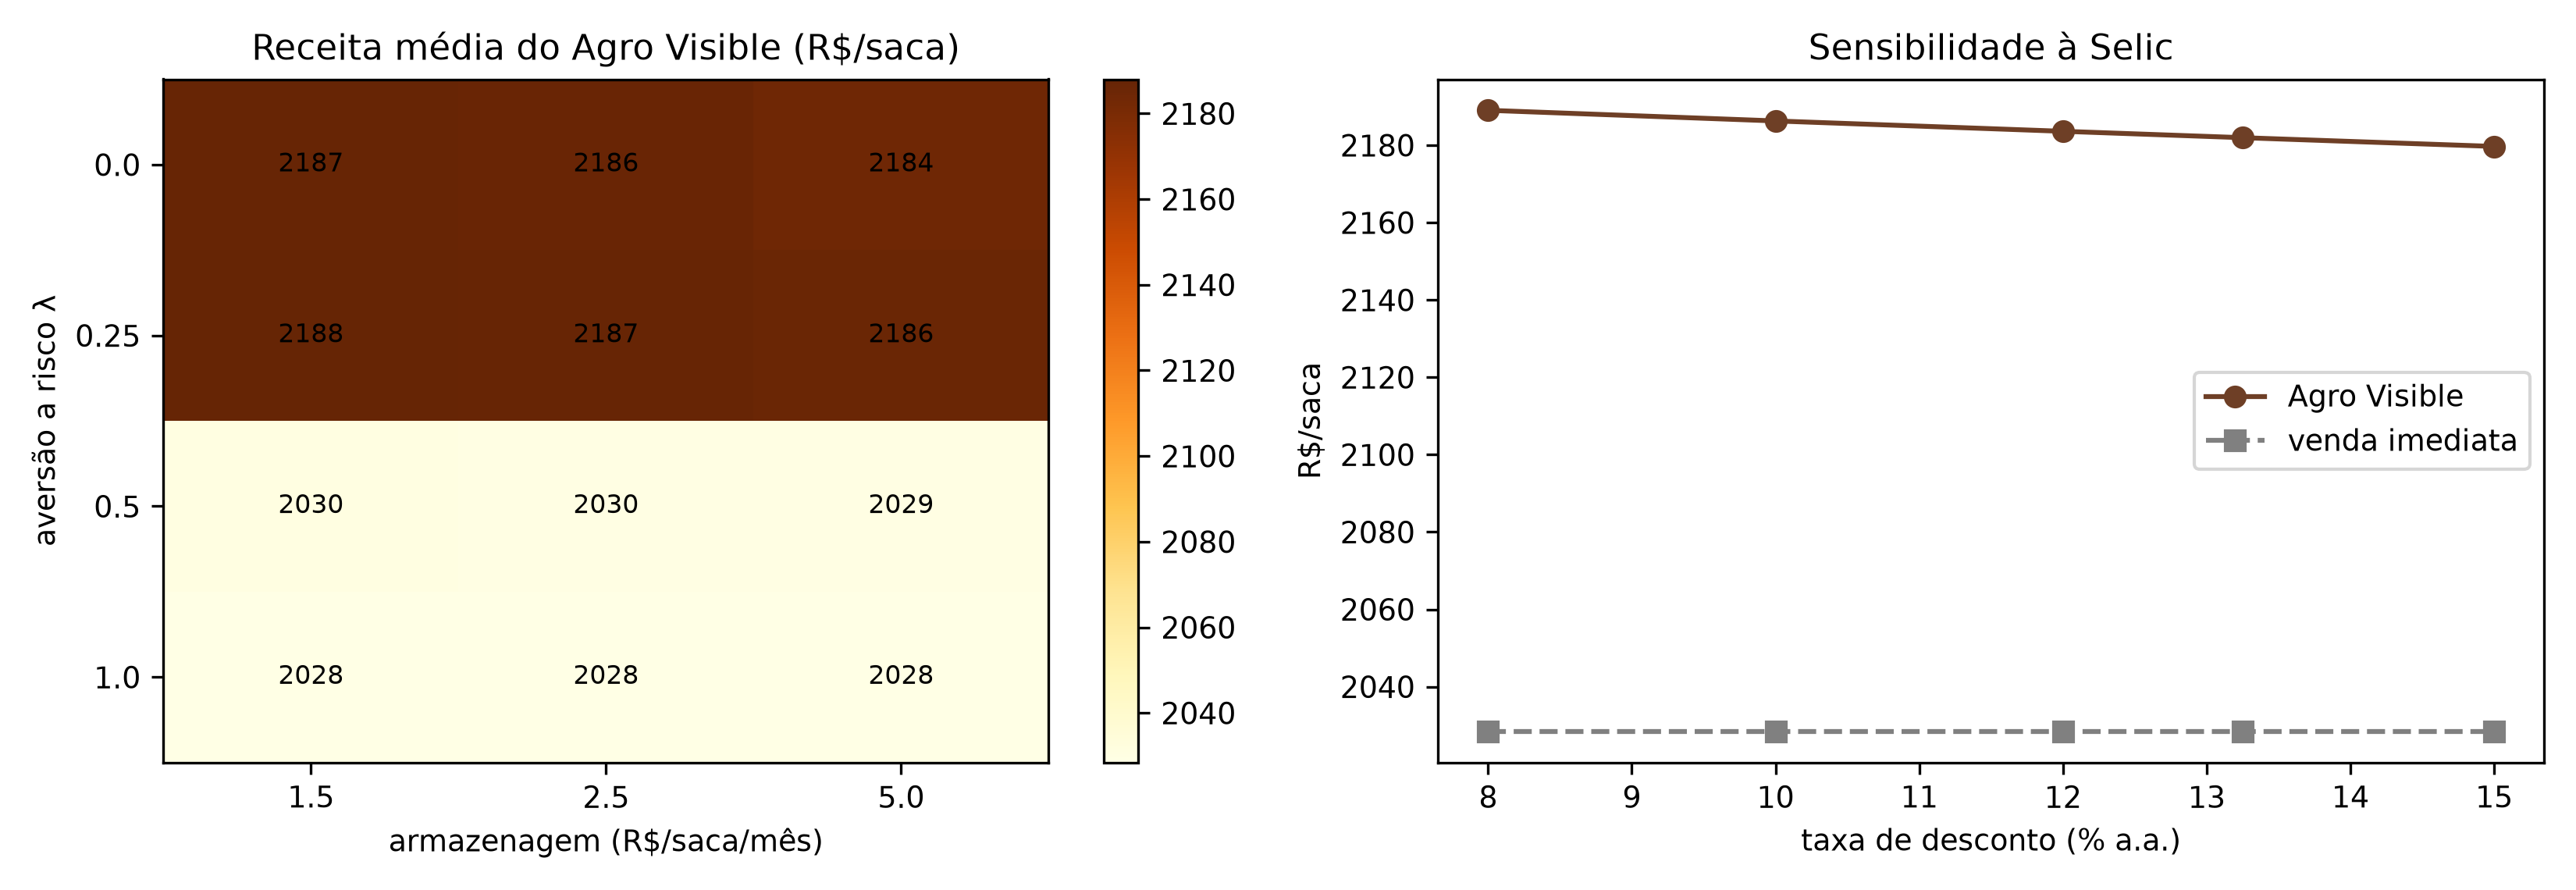
\includegraphics[width=\textwidth]{imgs/09_sensibilidade_lambda_armazenagem_selic.png}
	\fonte{Do autor (2026).}
\end{figure}

\paragraph{Taxa de desconto.} Entre 8 \% e 15 \% a.a., faixa que cobre toda a variação da Selic no período, a receita do AgroVisible move-se menos de 5 R\$/sc e nenhuma das 20 ações muda. O efeito da taxa é maior sobre a venda parcelada, que perde 31 R\$/sc na mesma faixa porque sempre carrega parte da produção por seis meses. A política é insensível à Selic porque as decisões de armazenar são tomadas quando a deriva prevista é de 10 a 20 \% em poucos meses, ordem de grandeza acima do custo de oportunidade mensal de cerca de 1 \%.

\paragraph{Armazenagem.} Entre 1,50 e 5,00 R\$/sc/mês a receita varia 2 R\$/sc e nenhuma ação muda. Com o preço da saca acima de 1\,300 R\$, a armazenagem mensal representa de 0,1 a 0,4 \% do valor, inferior ao custo de oportunidade e muito inferior à deriva prevista. Esse resultado também torna irrelevante a incerteza sobre o valor exato da tarifa de armazém, discutida no \autoref{sec:ameacas}.

\paragraph{Base e risco de base.} Com neutralidade a risco, deslocar a base esperada em 5 pontos percentuais para qualquer lado, ou dobrar o risco de base, não altera nenhuma decisão nem a receita. A razão é que a ação de \textit{hedge}, única afetada por esses parâmetros, nunca é competitiva no \textit{backtest}: com a curva de futuros aproximada pelo primeiro vencimento e o mercado em \textit{backwardation}, travar o preço futuro sempre rendia menos que vender ou armazenar descoberto. A base só passa a influenciar a política na recomendação corrente, em que a curva real por vencimento está disponível: na data de 31 de agosto de 2026, com a base em $-$26 \% contra $-$21 \% sazonal, o \textit{hedge} de um mês trava cerca de 1\,816 R\$/sc contra 1\,748 do físico e torna-se a ação recomendada para $\lambda$ entre 0,25 e 0,5.

\paragraph{Aversão a risco.} O único parâmetro que muda a política é $\lambda$. Até 0,5 a receita média permanece em 2\,079 a 2\,081 R\$/sc, mas a frequência de armazenar cai de 25 \% para 10 \% das datas: o produtor avesso a risco deixa de armazenar nas datas em que a deriva prevista é pequena diante da dispersão, e essas eram as datas de ganho marginal. Em $\lambda = 1$ o motor vende em 19 das 20 datas e a receita colapsa para a da venda imediata. A aversão a risco, portanto, não destrói o ganho da política até valores moderados; ela o concentra em menos decisões, cada uma com maior convicção. O desvio-padrão da receita entre datas, porém, cresce de 392 para 406 R\$/sc de $\lambda = 0$ a $\lambda = 1$, porque a venda imediata em um mercado volátil é, ela própria, a estratégia de maior dispersão entre datas.

\section{Custo computacional}\label{sec2:res-custo}

Em CPU, sem aceleração por GPU, o treino do modelo final levou 125 segundos; a resolução do motor de decisão para uma data, com sete camadas e 121 nós de preço, leva 2 milissegundos; o \textit{backtest} completo de 20 datas com política rolante, cerca de 120 resoluções do motor, leva 0,4 segundo. A grade de sensibilidade de 12 \textit{backtests} leva um minuto, e os 23 retreinos da ablação e do estudo de sementes levaram 35 minutos. O custo computacional da ferramenta é, portanto, compatível com execução em um computador pessoal ou em um servidor modesto de cooperativa, e a etapa cara, o treino da rede, precisa ser repetida apenas quando novos dados justificam.
